% !TeX spellcheck = ru_RU

\subsection{Генеративные состязательные сети}

Генеративные состязательные сети (\emph{Generative adversarial network}, сокр., \emph{GAN})  это семейство генеративных моделей, разработанное Яном Гудфеллоу в 2014 году \cite{goodfellow2014generative}.  Они формулируют процесс обучения  генеративной модели в виде антагонистической игры между двумя игроками: \emph{генератором} и \emph{дискриминатором}.

Генератор $G$ представляет собой глубокую нейронную сеть, задающую отбражение из латентного пространства $\mathcal Z$ в пространство данных $\mathcal X$.
Принимая на вход случайные вектора из некоторого заданного распределения $p(z)$ в $\mathcal Z$, он производит набор синтетических данных, пытаясь аппроксимировать распределение обучающей выборки $q_{data}(x)$.

% ... возвращает вероятность ...
Дискриминатор $D$ представляет собой глубокую нейронную сеть, задающую отбражение из пространства данных $\mathcal X$ в $\mathbb R$. Получив на вход некоторый элемент из пространства $\mathcal X$, дискриминатор возвращает значение, характеризующее вероятность того, что он был получен из распределения реальных данных $q_{data}(x)$, а не сгенерирован генератором $G$.

\begin{figure}[h]
\begin{center}
    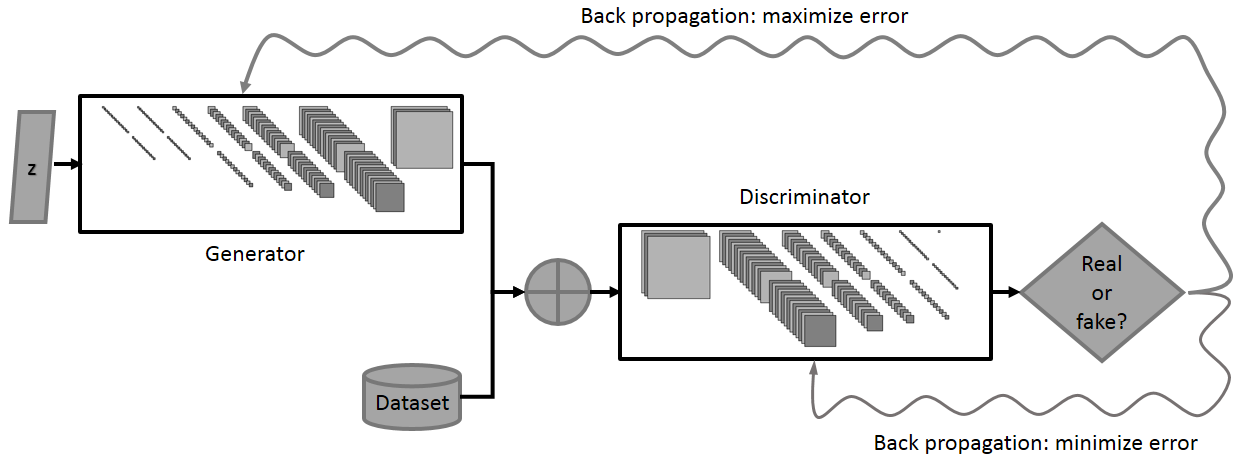
\includegraphics[width=0.9\textwidth]{gan}
    \caption{Архитектура генеративной состязательной сети.}
    \label{fig:subim11}
\end{center}
\end{figure}
% img src: https://blogs.nvidia.com/blog/2018/08/02/supervised-unsupervised-learning./

Роль дискриминатора состоит в том, чтобы как можно более точно отличать синтетические данные, полученные генератором, от реальных данный, взятых из обучающей выборки, в то время как генератор пытается обмануть дискриминатор путем генерирования синтетических данных, как можно более похожих на реальные.
Процесс совместного конкурентного обучения продолжается вплоть до достижения парой $(G, D)$ <<седловой точки>> (т.е. равновесия по Нэшу) \cite{goodfellow2017nips} функции выигрыша
$$
\min_{G} \max_{D} V(G, D) = \mathop{\mathbb{E}}_{x \sim q_{data}(x)} [\log D(x)] + \mathop{\mathbb{E}}_{z \sim p(z)} [\log (1 - D(G(z)))] ,
$$
в которой генератор способен генерировать данные, неотличимые дискриминатором от реальных.

\subsection{Генеративные нейронные сети для генерации лиц}

При решении задачи генерации изображений (в.т.ч. изображений лиц), пространство данных $\mathcal X$ предстваляет собой пространство изображений, каждый элемент которого обладает некоторым набором семантических признаков.
В случае лиц такими признаками могут являться положение головы, пол, возраст и т.д.

% семплированный -> взятый
Генератор $G$ является сверточной нейронной сетью, которая представляет собой композицию из $L$ сверточных слоев $G_1 ... G_L$ . 
Первый слой получает на вход случайный вектор $\mathbf z$, семплированный из многомерного нормального распределения $p(z)$ в латентном пространстве $\mathcal Z$, и возвращает тензор признаков $y_1 = G_1(\mathbf z)$. 
Каждый последующие слои применяется к выходам предыдущего: 
$$ y_i = G_i(y_{i-1}), $$
результатом применения последнего слоя является изображение $I = G_L(y_{L-1}) \equiv G(\mathbf z)$.

\subsubsection{BigGAN}
% TODO: абзац про то, что генерирование изобр. высокого разрешения - сложно

BigGAN \cite{bigGAN} --- генеративная состязательная сеть, спроектированная с целью масштабирования архитектуры для генерации изображений высокого разрешения.
BigGAN вносит ряд модификаций в стандартную архитектуру генеративных состязательных сетей.
Так, в архитектуру внедряются Skip\emph{-z} соединения, который позволяют промежучтоным слоям сети также принимать на вход латентный вектор:
$$ y_i = G_i(y_{i-1}, \mathbf z). $$
Кроме того, в архитектуре BigGAN применяются self-attention слой и спектральная нормализация весов.
Это позволяет увеличить количество весов модели в 2 раза и добиться качественной генерации изображений с разрешением до $512\times512$ на самых разнообразных классах изображений.

\subsubsection{StyleGAN}
StyleGAN \cite{StyleGAN} --– это генеративная состязательная сеть, архитектура которой разрабатывалась специально с целью генерации реалистичных изображений лиц.

% FIXME: linebreak
StyleGAN вводит промежуточное латентное пространство $\mathcal W$, предназначенное для решения проблемы кривизны, или "запутaнности" \linebreak (\emph{entanglement}), латентного пространства \cite{arvanitidis2018oddity}. 
Эта проблема возникает из-за ограничений и дефектов в вероятносном распределении тренировочных данных (рис. \ref{fig:stylegan-mapping}). 
Во время обучения StyleGAN выучивает нелинейное преобразование $M: \mathcal Z \mapsto \mathcal W$, которое позволяет избавиться от ограничений, накладываемых вероятносным распределением тренировочных данных, и получить более линейное латентное пространство.

\begin{figure}[h]
\begin{center}
    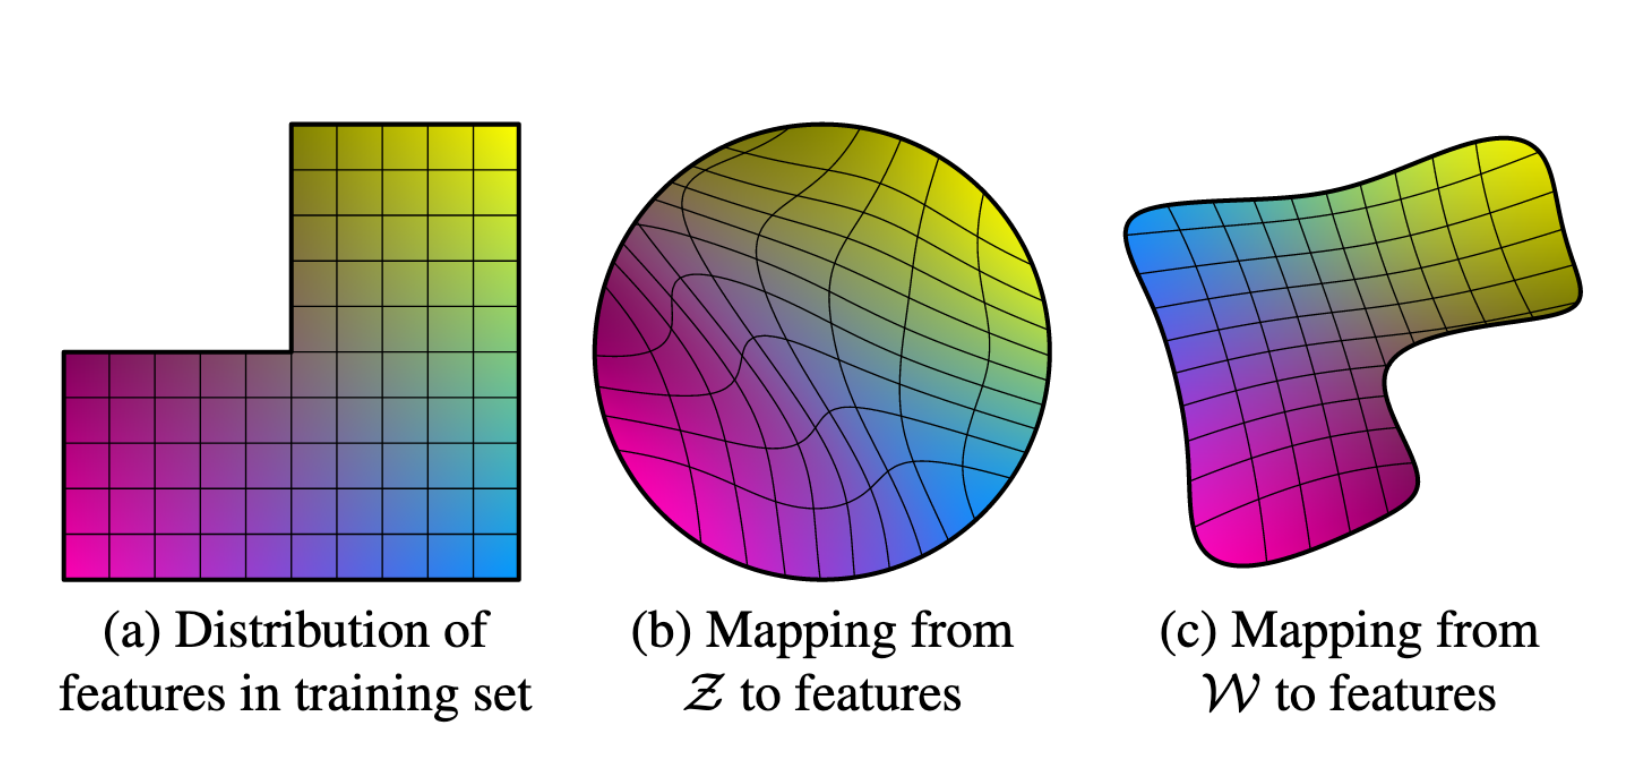
\includegraphics[width=0.7\textwidth]{stylegan_mapping}
    \caption{Иллюстрация действия промежуточного латентного пространства на примере двух факторов вариации (напр., \emph{пол} и \emph{наличие бороды}). Изображение взято из \cite{StyleGAN}.}
    \label{fig:stylegan-mapping}
    
    %FIXME: \small может лучше смотреться
    \footnotesize
 {(a)}~--- пример тренировочных данных, в которых отсутствует некоторая комбинация признаков; 
 {(b)}~--- это приводит к возникновению искривления отображения из $\mathcal Z$ в пространство признаков, которое исключает семплинг несуществующей комбинации из $\mathcal Z$;
 {(c)}~--- выучиваемое отображение из $\mathcal Z$ в $\mathcal W$ способно обратить данное искривление.

\end{center}
\end{figure}

StyleGAN модифицирует архитектуру генератора, основываясь на идеях из области Style Transfer. 
Синтез изображения начинается с фиксированного вектора $y_0$, а информация о латентном представлениии последовательно встраивается в каждый промежуточный слой генератора:
$$ y_i = G(y_{i-1}, \mathbf w),\quad \mathbf w = M(\mathbf z). $$
Это позволяет контролировать силу проявления различных семантических признаков изображения на разных масштабах, от грубых признаков, определяемых первыми слоями генератора, до тонких деталей, определяемых последними слоями.
В сочитании с встраиванием шума напрямую в слои сети, такая архитектура позволяет отделить высокоуровневые признаки изображения (положения лица, личность человека) от случайных вариационных факторов (волосы, веснушки и т.п.).

Кроме того, использование в каждом слое сети своего отдельного $\mathbf w_i$ позволяет производить операцию "смешивания стиля", комбинируя семантические признаки различных уровней абстракции с нескольких генерируемых изображений.

%TODO: как-то привести в именительный падеж
Дальнейшему улучшению данной архитектуры, StyleGAN2 \cite{karras2020stylegan2}, удалось добиться еще лучших результатов в задаче устранения "запутанности" латентного пространства и улучшения качества генерируемых изображений.
Кроме того, данной архитектурой также реализован алгоритм обратного отображения, названный StyleGAN2 Projector, который позволяет отобразить реальное изображение в латентное пространство сети.

\subsubsection{ALAE}
ALAE \cite{ALAE} –-- это генеративная нейронная сеть, архитектура которой разрабатывалась с целью предоставления возможности манипулирования латентными представлениями сети.

ALAE заимствует идеи вариационных автоэнкодеров \cite{kingma2014vae}, и дополняет стандартную архитектуру генеративных состязательных сетей энкодером $E$ и декодером $F$.
Декодер отображает входной латентный вектор в промежуточное латентное пространство $\mathcal W$, перед тем как подать его на вход генератору.
Энкодер отображает сгенерированное генератором изображение в промежуточное латентное пространство, перед тем как подать его на вход дискриминатору (рис. \ref{fig:alae}).

\begin{figure}[h]
\begin{center}
    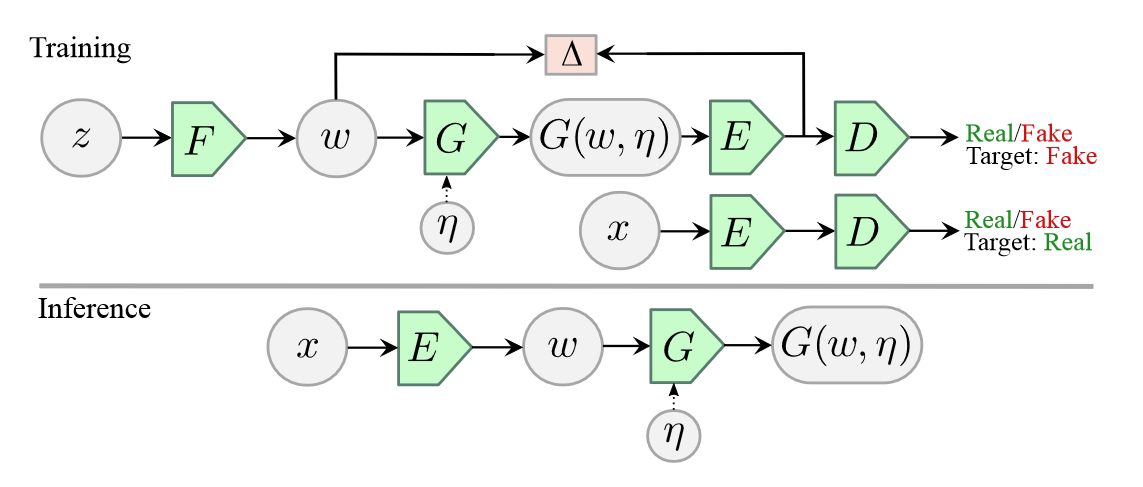
\includegraphics[width=0.9\textwidth]{ALAE}
    \caption{Архитектура ALAE. Изображение взято из \cite{ALAE}.}
    \label{fig:alae}
\end{center}
\end{figure}

В процессе обучения данная сеть применяет стратегию обучения автоэнкодеров, чтобы получить оптимальное латентное распределение в промежуточном латентном пространстве, накладывая ограничение о взаимной близости представлений, полученных энкодером и декодером;
и состязательную стратегию обучения, чтобы аппроксимировать распределение данных обучающей выборки.


\subsection{Алгоритмы отображения изображений в латентное пространство сети}

Для работы с реальными изображениями генеративным состязательным сетям требуется обратное отображение, позволяющее по входному изображению получить соответствующий ему латентный вектор в латентном пространстве сети. 
Классическая архитектура генеративных состязательных сетей не задает такого отображения напрямую, а потому для работы с реальными изображениями реализуются алгоритмы, позволяющие аппроксимировать данный латентный вектор.

Обучение дополнительного энкодера \cite{donahue2016adversarial} является распространенным подходом к нахождению обратного отображения.
Обратное отображение аппроксимируется нейронной сетью, которая обучается решению задачи регрессии латентного вектора по заданному входному изображению. 
Обучение энкодера производится на датасете пар <\emph{изображение, вектор}>, состоящем из набора синтетических изображений, сгенерированных генеративной состязательной сетью, и входных латентных векторов, с помощью которых это изображение было получено.

Латентная оптимизация \cite{perarnau2016invertible} --- это алгоритм приближения латентного вектора путем минимизации некоторой заданной функции потерь реконструкции.
Алгоритм определяет некоторую гладкую функцию потерь $loss(I_{real}, G(\mathbf z)) $, которая характеризует, насколько изображение, сгенерированное с помощью текщего латентного вектора $\mathbf z$, близко к входному изображению $I_{real}$.
Поскольку генератор $G(z)$ является отображением, дифференциируемым по входному вектору (благодаря методу обратного распространения ошибки), а его гладкость зависит главным образом от выбора гладких функций активации (т.к. он является композицией линейных слоев и функций активации), это позволяет минимизировать заданную функцию потерь методом градиентного спуска, итеративно обновляя латентный вектор.

Использование в качестве архитектуры генератора StyleGAN позволяет улучшить процесс латентной оптимизации.
Оптимизация в расширенном латентном пространстве $\mathcal W+$, которое представляет собой конкатенацию 18 различных векторов $\mathbf w_i$, поступающих на вход каждому отдельному слою архитектуры StyleGAN, позволяет получить более точную реконструкцию входного изображения \cite{abdal2019image2stylegan}.


\subsection{Алгоритмы выделения семантик изображения в латентном пространстве сети}

Идея манипулирования латентным вектором для изменения семантических признаков генерируемых изображений основана на наблюдении о том, что к латентным векторам применима векторная арифметика \cite{radford2015unsupervised}.

Многие исследования латентных пространств генеративных состязательных сетей исходят их предположения о том, что отдельные факторы вариации генерируемых изображений контролируются некоторыми одномерными линейными подпространствами латентного пространства сети \cite{StyleGAN}.
Таким образом, зная базисный вектор подпространства, соответствующего определенному семантическому признаку, можно добиться увеличения или уменьшения выраженности данного признака на сгенерированном изображении путем линейного сдвига латентного вектора в направлении данного базисного вектора \cite{abdal2019image2stylegan}. 
Далее данный вектор будем называть \emph{семантическим вектором признака} в латентном пространстве генеративной состязательной сети.

GANSpace \cite{hrknen2020ganspace} --- это фреймворк, предназначенный для выделения и анализа семантических векторов, и использования их для редактирования семантических признаков на генерируемом изображении.
Для выделения семантических векторов данным фреймворком реализуется алгоритм, базирующийся на методе главных компонент.
Он применяет метод главных компонент для уменьшения размерности латентного пространства и выделения в нем наиболее значимых направлений. Эти направления принимаются в качестве базисных векторов, и дальнейший визуальный анализ изменений, которые вызывает линейный сдвиг по данным направлениям на генерируемых изображениях, показывает, каким семантическим признакам эти направления соответствуют.

InterFaceGAN \cite{shen2020interfacegan} --- это фреймворк, нацеленный на более контролируемое исследование латентного пространства генеративной состязательной сети.
Он ставит своей задачей нахождение того, как в латентное пространство отображается некоторый бинарный семантический признак, заданный набором пооложительных и отрицательных примеров.
Для этого фреймворком InterFaceGAN реализуется одноименный алгоритм выделения семантических векторов.
Этот алгоритм базируется на обозначенном в \cite{StyleGAN} факте о том, что два набора латентных векторов, соответствующих изображениям с различными значениями некоторого бинарного семантического признака, будут линейно разделимы в латентном пространстве.
Нахождение семантического вектора заданного бинарного признака сводится к нахождению оптимальной разделяющей гиперплоскости между данными наборами латентных векторов.
В качестве семантического вектора берется нормальный вектор найденной гиперплоскости.
